\documentclass[a4paper]{book}
\usepackage{a4wide}
\usepackage{makeidx}
\usepackage{graphicx}
\usepackage{multicol}
\usepackage{float}
\usepackage{listings}
\usepackage{color}
\usepackage{textcomp}
\usepackage{alltt}
\usepackage{times}
\usepackage{ifpdf}
\ifpdf
\usepackage[pdftex,
            pagebackref=true,
            colorlinks=true,
            linkcolor=blue,
            unicode
           ]{hyperref}
\else
\usepackage[ps2pdf,
            pagebackref=true,
            colorlinks=true,
            linkcolor=blue,
            unicode
           ]{hyperref}
\usepackage{pspicture}
\fi
\usepackage[utf8]{inputenc}
\usepackage{doxygen}
\lstset{language=C++,inputencoding=utf8,basicstyle=\footnotesize,breaklines=true,breakatwhitespace=true,tabsize=8,numbers=left }
\makeindex
\setcounter{tocdepth}{3}
\renewcommand{\footrulewidth}{0.4pt}
\begin{document}
\hypersetup{pageanchor=false}
\begin{titlepage}
\vspace*{7cm}
\begin{center}
{\Large Reference Manual}\\
\vspace*{1cm}
{\large Generated by Doxygen 1.7.1}\\
\vspace*{0.5cm}
{\small Tue Feb 15 2011 12:38:27}\\
\end{center}
\end{titlepage}
\clearemptydoublepage
\pagenumbering{roman}
\tableofcontents
\clearemptydoublepage
\pagenumbering{arabic}
\hypersetup{pageanchor=true}
\chapter{Class Index}
\section{Class Hierarchy}
This inheritance list is sorted roughly, but not completely, alphabetically:\begin{DoxyCompactList}
\item \contentsline{section}{BaseAI}{\pageref{classBaseAI}}{}
\begin{DoxyCompactList}
\item \contentsline{section}{AI}{\pageref{classAI}}{}
\end{DoxyCompactList}
\item \contentsline{section}{Client}{\pageref{interfaceClient}}{}
\item \contentsline{section}{ExistentialError}{\pageref{classExistentialError}}{}
\item \contentsline{section}{Main}{\pageref{classMain}}{}
\item \contentsline{section}{Move}{\pageref{classMove}}{}
\item \contentsline{section}{Piece}{\pageref{classPiece}}{}
\end{DoxyCompactList}

\chapter{Class Index}
\section{Class List}
Here are the classes, structs, unions and interfaces with brief descriptions:\begin{DoxyCompactList}
\item\contentsline{section}{\hyperlink{classAI}{AI} (The class implementing gameplay logic )}{\pageref{classAI}}{}
\item\contentsline{section}{\hyperlink{classBaseAI}{BaseAI} (A basic \hyperlink{classAI}{AI} interface )}{\pageref{classBaseAI}}{}
\item\contentsline{section}{\hyperlink{interfaceClient}{Client} }{\pageref{interfaceClient}}{}
\item\contentsline{section}{\hyperlink{classExistentialError}{ExistentialError} }{\pageref{classExistentialError}}{}
\item\contentsline{section}{\hyperlink{classMain}{Main} }{\pageref{classMain}}{}
\item\contentsline{section}{\hyperlink{classMove}{Move} (A chess move )}{\pageref{classMove}}{}
\item\contentsline{section}{\hyperlink{classPiece}{Piece} (A chess piece )}{\pageref{classPiece}}{}
\end{DoxyCompactList}

\chapter{Class Documentation}
\hypertarget{classAI}{
\section{AI Class Reference}
\label{classAI}\index{AI@{AI}}
}


The class implementing gameplay logic.  


Inheritance diagram for AI:\begin{figure}[H]
\begin{center}
\leavevmode
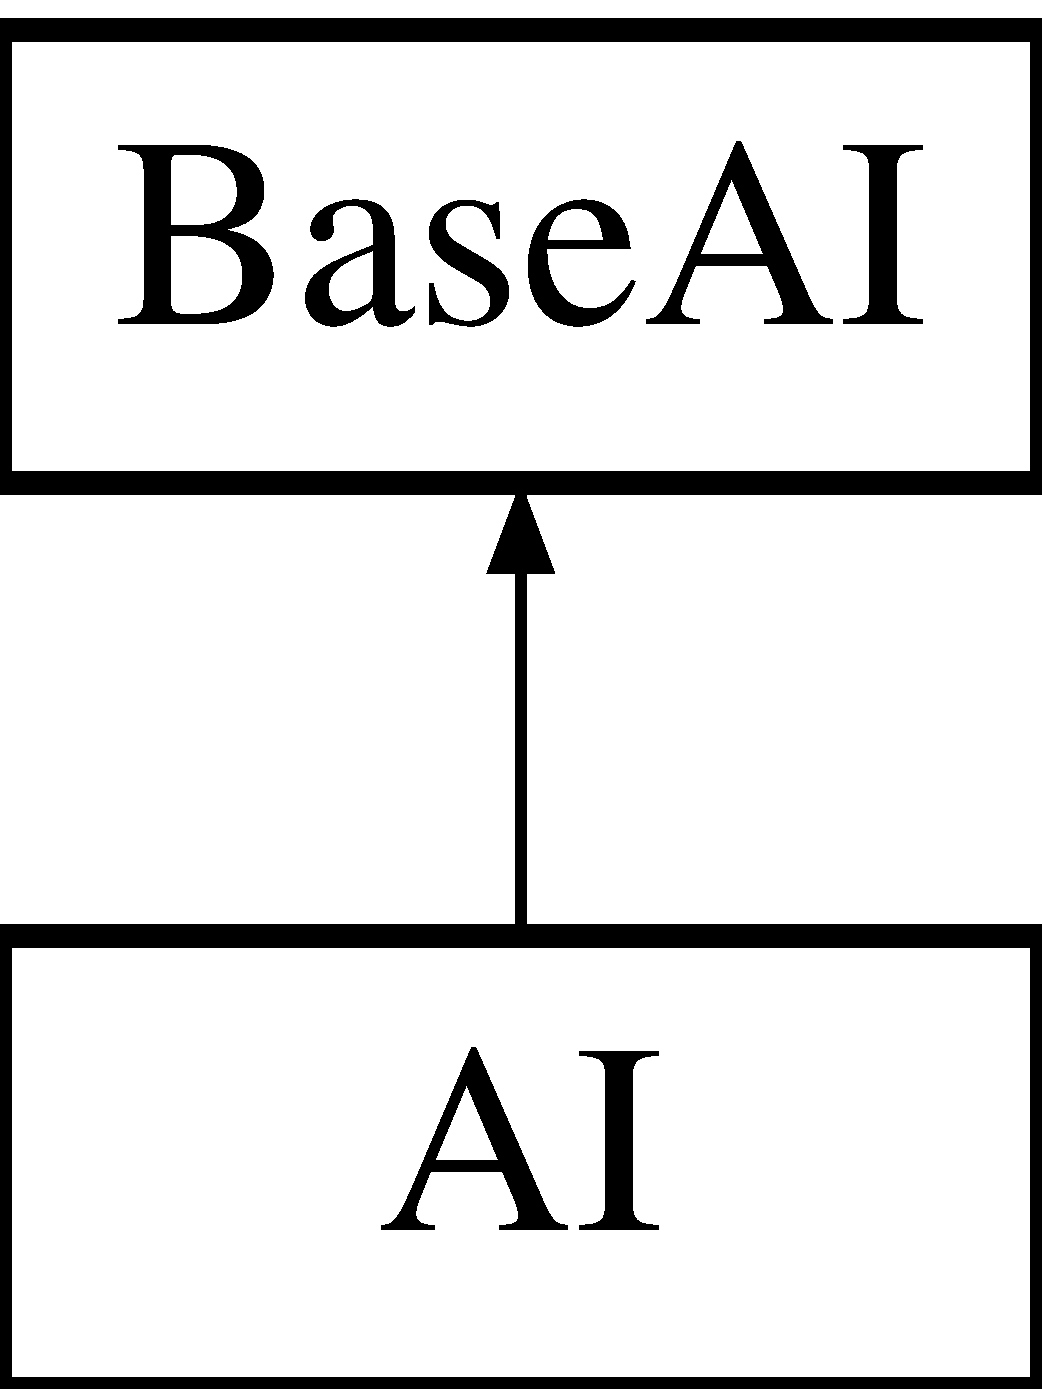
\includegraphics[height=2.000000cm]{classAI}
\end{center}
\end{figure}
\subsection*{Public Member Functions}
\begin{DoxyCompactItemize}
\item 
String \hyperlink{classAI_ad7e6db6b414a192ad2af8656d012cfdc}{username} ()
\item 
String \hyperlink{classAI_a405047fd39e03de993183392a06d655b}{password} ()
\item 
boolean \hyperlink{classAI_af25b3a076daef2aaf9f74ecf458bdfbc}{run} ()
\item 
void \hyperlink{classAI_a8c8e3a635791abaa61585357e6a25f63}{init} ()
\item 
void \hyperlink{classAI_a67b00a8dd5c6d73db2e4e2332826462e}{end} ()
\item 
\hypertarget{classAI_a8487ba177f1c1431a134c2b56b94ad8b}{
{\bfseries AI} (Pointer c)}
\label{classAI_a8487ba177f1c1431a134c2b56b94ad8b}

\end{DoxyCompactItemize}


\subsection{Detailed Description}
The class implementing gameplay logic. 

\subsection{Member Function Documentation}
\hypertarget{classAI_a67b00a8dd5c6d73db2e4e2332826462e}{
\index{AI@{AI}!end@{end}}
\index{end@{end}!AI@{AI}}
\subsubsection[{end}]{\setlength{\rightskip}{0pt plus 5cm}void AI::end (
\begin{DoxyParamCaption}
{}
\end{DoxyParamCaption}
)\hspace{0.3cm}{\ttfamily  \mbox{[}inline, virtual\mbox{]}}}}
\label{classAI_a67b00a8dd5c6d73db2e4e2332826462e}
This is run on after your last turn. 

Implements \hyperlink{classBaseAI_afb1c3a00ed081e9efdfff9f7d1e6910d}{BaseAI}.

\hypertarget{classAI_a8c8e3a635791abaa61585357e6a25f63}{
\index{AI@{AI}!init@{init}}
\index{init@{init}!AI@{AI}}
\subsubsection[{init}]{\setlength{\rightskip}{0pt plus 5cm}void AI::init (
\begin{DoxyParamCaption}
{}
\end{DoxyParamCaption}
)\hspace{0.3cm}{\ttfamily  \mbox{[}inline, virtual\mbox{]}}}}
\label{classAI_a8c8e3a635791abaa61585357e6a25f63}
This is run on turn 1 before run 

Implements \hyperlink{classBaseAI_a71b49f4ca248bfd32a9f9557cb6d494a}{BaseAI}.

\hypertarget{classAI_a405047fd39e03de993183392a06d655b}{
\index{AI@{AI}!password@{password}}
\index{password@{password}!AI@{AI}}
\subsubsection[{password}]{\setlength{\rightskip}{0pt plus 5cm}String AI::password (
\begin{DoxyParamCaption}
{}
\end{DoxyParamCaption}
)\hspace{0.3cm}{\ttfamily  \mbox{[}inline, virtual\mbox{]}}}}
\label{classAI_a405047fd39e03de993183392a06d655b}
Make this your password, which should be provided. 

Implements \hyperlink{classBaseAI_a8607533e2b5bd9920ded593ae6509f48}{BaseAI}.

\hypertarget{classAI_af25b3a076daef2aaf9f74ecf458bdfbc}{
\index{AI@{AI}!run@{run}}
\index{run@{run}!AI@{AI}}
\subsubsection[{run}]{\setlength{\rightskip}{0pt plus 5cm}boolean AI::run (
\begin{DoxyParamCaption}
{}
\end{DoxyParamCaption}
)\hspace{0.3cm}{\ttfamily  \mbox{[}inline, virtual\mbox{]}}}}
\label{classAI_af25b3a076daef2aaf9f74ecf458bdfbc}
This is run every turn . Return true to end the turn, return false to request a status update from the server and then immediately rerun this function with the latest game status. 

Implements \hyperlink{classBaseAI_a56c96a58c1f1e93d17f9817711a45594}{BaseAI}.

\hypertarget{classAI_ad7e6db6b414a192ad2af8656d012cfdc}{
\index{AI@{AI}!username@{username}}
\index{username@{username}!AI@{AI}}
\subsubsection[{username}]{\setlength{\rightskip}{0pt plus 5cm}String AI::username (
\begin{DoxyParamCaption}
{}
\end{DoxyParamCaption}
)\hspace{0.3cm}{\ttfamily  \mbox{[}inline, virtual\mbox{]}}}}
\label{classAI_ad7e6db6b414a192ad2af8656d012cfdc}
Make this your username, which should be provided. 

Implements \hyperlink{classBaseAI_aa26770dd7db8dd0c4466dd770d4e05ba}{BaseAI}.



The documentation for this class was generated from the following file:\begin{DoxyCompactItemize}
\item 
AI.java\end{DoxyCompactItemize}

\hypertarget{classBaseAI}{
\section{BaseAI Class Reference}
\label{classBaseAI}\index{BaseAI@{BaseAI}}
}


A basic \hyperlink{classAI}{AI} interface.  


Inheritance diagram for BaseAI:\begin{figure}[H]
\begin{center}
\leavevmode
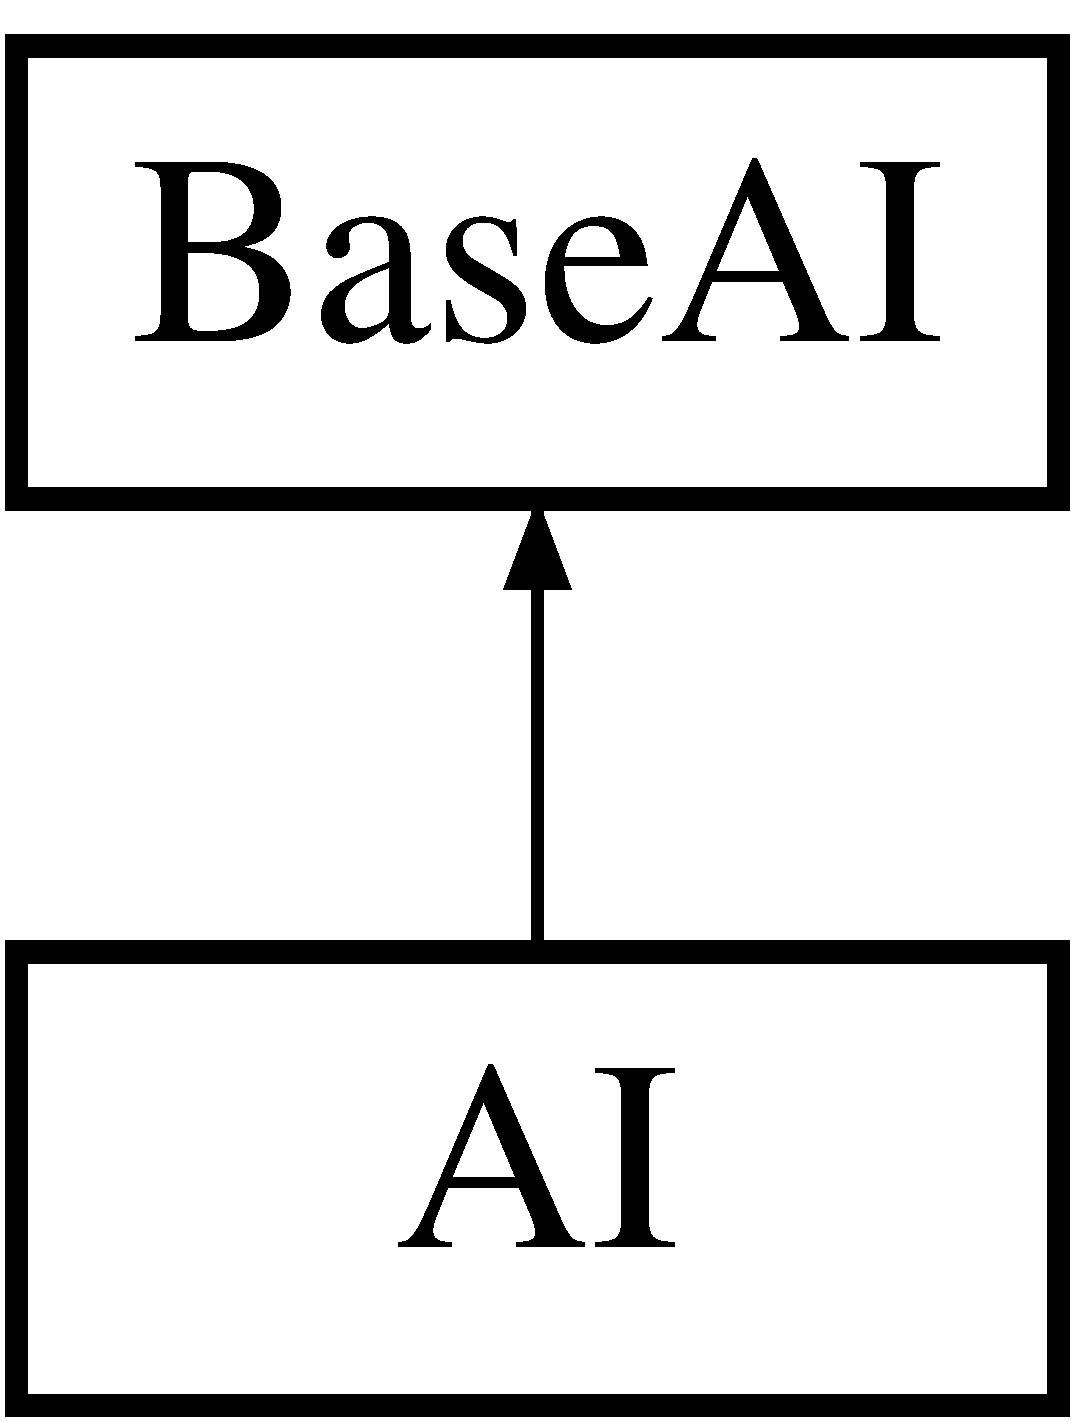
\includegraphics[height=2.000000cm]{classBaseAI}
\end{center}
\end{figure}
\subsection*{Public Member Functions}
\begin{DoxyCompactItemize}
\item 
\hypertarget{classBaseAI_a27e93801ded2a4e1846f2b58beb37972}{
{\bfseries BaseAI} (Pointer c)}
\label{classBaseAI_a27e93801ded2a4e1846f2b58beb37972}

\item 
abstract String \hyperlink{classBaseAI_aa26770dd7db8dd0c4466dd770d4e05ba}{username} ()
\item 
abstract String \hyperlink{classBaseAI_a8607533e2b5bd9920ded593ae6509f48}{password} ()
\item 
abstract void \hyperlink{classBaseAI_a71b49f4ca248bfd32a9f9557cb6d494a}{init} ()
\item 
abstract boolean \hyperlink{classBaseAI_a56c96a58c1f1e93d17f9817711a45594}{run} ()
\item 
abstract void \hyperlink{classBaseAI_afb1c3a00ed081e9efdfff9f7d1e6910d}{end} ()
\item 
\hypertarget{classBaseAI_a862e05b3099817fcceb55beeef7225fe}{
boolean {\bfseries startTurn} ()}
\label{classBaseAI_a862e05b3099817fcceb55beeef7225fe}

\end{DoxyCompactItemize}
\subsection*{Package Functions}
\begin{DoxyCompactItemize}
\item 
\hypertarget{classBaseAI_a19ade7391bfe101884a35f48fb840199}{
int \hyperlink{classBaseAI_a19ade7391bfe101884a35f48fb840199}{turnNumber} ()}
\label{classBaseAI_a19ade7391bfe101884a35f48fb840199}

\begin{DoxyCompactList}\small\item\em How many turns it has been since the beginning of the game. \item\end{DoxyCompactList}\item 
\hypertarget{classBaseAI_a16aab1036653c8f8fb5370cf2f6a3e10}{
int \hyperlink{classBaseAI_a16aab1036653c8f8fb5370cf2f6a3e10}{playerID} ()}
\label{classBaseAI_a16aab1036653c8f8fb5370cf2f6a3e10}

\begin{DoxyCompactList}\small\item\em Player Number; either 0 or 1. \item\end{DoxyCompactList}\item 
\hypertarget{classBaseAI_a50d3091db33b93c6f7c2d11dd64b4c7a}{
int \hyperlink{classBaseAI_a50d3091db33b93c6f7c2d11dd64b4c7a}{gameNumber} ()}
\label{classBaseAI_a50d3091db33b93c6f7c2d11dd64b4c7a}

\begin{DoxyCompactList}\small\item\em What number game this is for the server. \item\end{DoxyCompactList}\item 
\hypertarget{classBaseAI_a21e92638c7b53df6bbb2116c1f0f51c7}{
int \hyperlink{classBaseAI_a21e92638c7b53df6bbb2116c1f0f51c7}{TurnsToStalemate} ()}
\label{classBaseAI_a21e92638c7b53df6bbb2116c1f0f51c7}

\begin{DoxyCompactList}\small\item\em How many turns until the game ends because no pawn has moved and no piece has been taken. \item\end{DoxyCompactList}\item 
\hypertarget{classBaseAI_a0c98c065f57b1519d6daf72ef1c71d71}{
int \hyperlink{classBaseAI_a0c98c065f57b1519d6daf72ef1c71d71}{player0Time} ()}
\label{classBaseAI_a0c98c065f57b1519d6daf72ef1c71d71}

\begin{DoxyCompactList}\small\item\em Player 0's time remaining. \item\end{DoxyCompactList}\item 
\hypertarget{classBaseAI_a5a96b2451bf0e2f6567e9e56d59cf7cb}{
int \hyperlink{classBaseAI_a5a96b2451bf0e2f6567e9e56d59cf7cb}{player1Time} ()}
\label{classBaseAI_a5a96b2451bf0e2f6567e9e56d59cf7cb}

\begin{DoxyCompactList}\small\item\em Player 1's time remaining. \item\end{DoxyCompactList}\end{DoxyCompactItemize}
\subsection*{Package Attributes}
\begin{DoxyCompactItemize}
\item 
\hypertarget{classBaseAI_ad9836b270a011daee8411f84590ba35a}{
Pointer {\bfseries connection}}
\label{classBaseAI_ad9836b270a011daee8411f84590ba35a}

\item 
\hypertarget{classBaseAI_a94966bbfdac0d091a7332f19b29935c3}{
boolean {\bfseries initialized}}
\label{classBaseAI_a94966bbfdac0d091a7332f19b29935c3}

\end{DoxyCompactItemize}
\subsection*{Static Package Attributes}
\begin{DoxyCompactItemize}
\item 
\hypertarget{classBaseAI_a60272155e436cb8537f3818db02772eb}{
static \hyperlink{classMove}{Move}\mbox{[}$\,$\mbox{]} {\bfseries moves}}
\label{classBaseAI_a60272155e436cb8537f3818db02772eb}

\item 
\hypertarget{classBaseAI_ab75d25237ef50c6f70ad8387718aa133}{
static \hyperlink{classPiece}{Piece}\mbox{[}$\,$\mbox{]} {\bfseries pieces}}
\label{classBaseAI_ab75d25237ef50c6f70ad8387718aa133}

\item 
\hypertarget{classBaseAI_ad7942cee117a347f7cb841ff4800408f}{
static int {\bfseries iteration}}
\label{classBaseAI_ad7942cee117a347f7cb841ff4800408f}

\end{DoxyCompactItemize}


\subsection{Detailed Description}
A basic \hyperlink{classAI}{AI} interface. This class implements most the code an \hyperlink{classAI}{AI} would need to interface with the lower-\/level game code. AIs should extend this class to get a lot of builer-\/plate code out of the way The provided \hyperlink{classAI}{AI} class does just that. 

\subsection{Member Function Documentation}
\hypertarget{classBaseAI_afb1c3a00ed081e9efdfff9f7d1e6910d}{
\index{BaseAI@{BaseAI}!end@{end}}
\index{end@{end}!BaseAI@{BaseAI}}
\subsubsection[{end}]{\setlength{\rightskip}{0pt plus 5cm}abstract void BaseAI::end (
\begin{DoxyParamCaption}
{}
\end{DoxyParamCaption}
)\hspace{0.3cm}{\ttfamily  \mbox{[}pure virtual\mbox{]}}}}
\label{classBaseAI_afb1c3a00ed081e9efdfff9f7d1e6910d}
This is run on after your last turn. 

Implemented in \hyperlink{classAI_a67b00a8dd5c6d73db2e4e2332826462e}{AI}.

\hypertarget{classBaseAI_a71b49f4ca248bfd32a9f9557cb6d494a}{
\index{BaseAI@{BaseAI}!init@{init}}
\index{init@{init}!BaseAI@{BaseAI}}
\subsubsection[{init}]{\setlength{\rightskip}{0pt plus 5cm}abstract void BaseAI::init (
\begin{DoxyParamCaption}
{}
\end{DoxyParamCaption}
)\hspace{0.3cm}{\ttfamily  \mbox{[}pure virtual\mbox{]}}}}
\label{classBaseAI_a71b49f4ca248bfd32a9f9557cb6d494a}
This is run on turn 1 before run 

Implemented in \hyperlink{classAI_a8c8e3a635791abaa61585357e6a25f63}{AI}.

\hypertarget{classBaseAI_a8607533e2b5bd9920ded593ae6509f48}{
\index{BaseAI@{BaseAI}!password@{password}}
\index{password@{password}!BaseAI@{BaseAI}}
\subsubsection[{password}]{\setlength{\rightskip}{0pt plus 5cm}abstract String BaseAI::password (
\begin{DoxyParamCaption}
{}
\end{DoxyParamCaption}
)\hspace{0.3cm}{\ttfamily  \mbox{[}pure virtual\mbox{]}}}}
\label{classBaseAI_a8607533e2b5bd9920ded593ae6509f48}
Make this your password, which should be provided. 

Implemented in \hyperlink{classAI_a405047fd39e03de993183392a06d655b}{AI}.

\hypertarget{classBaseAI_a56c96a58c1f1e93d17f9817711a45594}{
\index{BaseAI@{BaseAI}!run@{run}}
\index{run@{run}!BaseAI@{BaseAI}}
\subsubsection[{run}]{\setlength{\rightskip}{0pt plus 5cm}abstract boolean BaseAI::run (
\begin{DoxyParamCaption}
{}
\end{DoxyParamCaption}
)\hspace{0.3cm}{\ttfamily  \mbox{[}pure virtual\mbox{]}}}}
\label{classBaseAI_a56c96a58c1f1e93d17f9817711a45594}
This is run every turn . Return true to end the turn, return false to request a status update from the server and then immediately rerun this function with the latest game status. 

Implemented in \hyperlink{classAI_af25b3a076daef2aaf9f74ecf458bdfbc}{AI}.

\hypertarget{classBaseAI_aa26770dd7db8dd0c4466dd770d4e05ba}{
\index{BaseAI@{BaseAI}!username@{username}}
\index{username@{username}!BaseAI@{BaseAI}}
\subsubsection[{username}]{\setlength{\rightskip}{0pt plus 5cm}abstract String BaseAI::username (
\begin{DoxyParamCaption}
{}
\end{DoxyParamCaption}
)\hspace{0.3cm}{\ttfamily  \mbox{[}pure virtual\mbox{]}}}}
\label{classBaseAI_aa26770dd7db8dd0c4466dd770d4e05ba}
Make this your username, which should be provided. 

Implemented in \hyperlink{classAI_ad7e6db6b414a192ad2af8656d012cfdc}{AI}.



The documentation for this class was generated from the following file:\begin{DoxyCompactItemize}
\item 
BaseAI.java\end{DoxyCompactItemize}

\hypertarget{interfaceClient}{
\section{Client Interface Reference}
\label{interfaceClient}\index{Client@{Client}}
}


Inherits com::sun::jna::Library.

\subsection*{Public Member Functions}
\begin{DoxyCompactItemize}
\item 
\hypertarget{interfaceClient_a6d25aca960b1e1a38ce203d6a969f9bc}{
Pointer {\bfseries createConnection} ()}
\label{interfaceClient_a6d25aca960b1e1a38ce203d6a969f9bc}

\item 
\hypertarget{interfaceClient_acfc9ada4dc1c3c147bd10d33a93cd5d5}{
boolean {\bfseries serverConnect} (Pointer connection, String host, String port)}
\label{interfaceClient_acfc9ada4dc1c3c147bd10d33a93cd5d5}

\item 
\hypertarget{interfaceClient_a889a9d7b3e68cb21ffcfaa7b2c19861b}{
boolean {\bfseries serverLogin} (Pointer connection, String username, String password)}
\label{interfaceClient_a889a9d7b3e68cb21ffcfaa7b2c19861b}

\item 
\hypertarget{interfaceClient_a4912adbddcbeff19d01f001ccd210375}{
int {\bfseries createGame} (Pointer connection)}
\label{interfaceClient_a4912adbddcbeff19d01f001ccd210375}

\item 
\hypertarget{interfaceClient_a8a9bed85e15f075bee07458a87645b6b}{
int {\bfseries joinGame} (Pointer connection, int id)}
\label{interfaceClient_a8a9bed85e15f075bee07458a87645b6b}

\item 
\hypertarget{interfaceClient_aff558de8ad20a23858ce3dc165fc4db7}{
void {\bfseries endTurn} (Pointer connection)}
\label{interfaceClient_aff558de8ad20a23858ce3dc165fc4db7}

\item 
\hypertarget{interfaceClient_a64de0e135006bec1aa4875ab0760f691}{
void {\bfseries getStatus} (Pointer connection)}
\label{interfaceClient_a64de0e135006bec1aa4875ab0760f691}

\item 
\hypertarget{interfaceClient_a88dd14b60667b07d577798e1c707c05f}{
int {\bfseries networkLoop} (Pointer connection)}
\label{interfaceClient_a88dd14b60667b07d577798e1c707c05f}

\item 
\hypertarget{interfaceClient_ae6117daed1d85523cbede25e9ca8632b}{
int {\bfseries pieceMove} (Pointer object, int file, int rank, int type)}
\label{interfaceClient_ae6117daed1d85523cbede25e9ca8632b}

\item 
\hypertarget{interfaceClient_a1c180b84ed7e74644ac62c1e069e26de}{
int {\bfseries getTurnNumber} (Pointer connection)}
\label{interfaceClient_a1c180b84ed7e74644ac62c1e069e26de}

\item 
\hypertarget{interfaceClient_a45ca933e037a2fa5ce4f97e67eb8b62f}{
int {\bfseries getPlayerID} (Pointer connection)}
\label{interfaceClient_a45ca933e037a2fa5ce4f97e67eb8b62f}

\item 
\hypertarget{interfaceClient_a172426923fb5bd5bdf79a3a3b6caf2e1}{
int {\bfseries getGameNumber} (Pointer connection)}
\label{interfaceClient_a172426923fb5bd5bdf79a3a3b6caf2e1}

\item 
\hypertarget{interfaceClient_a384c1a09c5026e955b79335561a61361}{
int {\bfseries getTurnsToStalemate} (Pointer connection)}
\label{interfaceClient_a384c1a09c5026e955b79335561a61361}

\item 
\hypertarget{interfaceClient_a1f16fbd34fbdee312db08c06d996b98b}{
int {\bfseries getPlayer0Time} (Pointer connection)}
\label{interfaceClient_a1f16fbd34fbdee312db08c06d996b98b}

\item 
\hypertarget{interfaceClient_a2996321a7d00f9179b4bf2b5e7b15665}{
int {\bfseries getPlayer1Time} (Pointer connection)}
\label{interfaceClient_a2996321a7d00f9179b4bf2b5e7b15665}

\item 
\hypertarget{interfaceClient_aa80bcad3cc5675a5636d2e6594fe41d8}{
Pointer {\bfseries getMove} (Pointer connection, int num)}
\label{interfaceClient_aa80bcad3cc5675a5636d2e6594fe41d8}

\item 
\hypertarget{interfaceClient_a03708130a71ab494fd548cdd0fae8174}{
int {\bfseries getMoveCount} (Pointer connection)}
\label{interfaceClient_a03708130a71ab494fd548cdd0fae8174}

\item 
\hypertarget{interfaceClient_a96ec2ddbbb75fdd44e4b0689ef9d901f}{
Pointer {\bfseries getPiece} (Pointer connection, int num)}
\label{interfaceClient_a96ec2ddbbb75fdd44e4b0689ef9d901f}

\item 
\hypertarget{interfaceClient_a8a8f318d62176bdfe0ddc7c776270fca}{
int {\bfseries getPieceCount} (Pointer connection)}
\label{interfaceClient_a8a8f318d62176bdfe0ddc7c776270fca}

\item 
\hypertarget{interfaceClient_ad3dfc9cd293e85e0f21c8dbaf89200f8}{
int {\bfseries moveGetId} (Pointer ptr)}
\label{interfaceClient_ad3dfc9cd293e85e0f21c8dbaf89200f8}

\item 
\hypertarget{interfaceClient_a7a86558ad65c59660e44c9e4c6d2815f}{
int {\bfseries moveGetFromFile} (Pointer ptr)}
\label{interfaceClient_a7a86558ad65c59660e44c9e4c6d2815f}

\item 
\hypertarget{interfaceClient_a164f5f09dd3aaaa20f3dd6199dd0d834}{
int {\bfseries moveGetFromRank} (Pointer ptr)}
\label{interfaceClient_a164f5f09dd3aaaa20f3dd6199dd0d834}

\item 
\hypertarget{interfaceClient_ac57c7a56bedebd47d82be8e9ee38e4e8}{
int {\bfseries moveGetToFile} (Pointer ptr)}
\label{interfaceClient_ac57c7a56bedebd47d82be8e9ee38e4e8}

\item 
\hypertarget{interfaceClient_ade447dc92d6b0a8e391f663474296f3b}{
int {\bfseries moveGetToRank} (Pointer ptr)}
\label{interfaceClient_ade447dc92d6b0a8e391f663474296f3b}

\item 
\hypertarget{interfaceClient_a5a83ce746d5752f1e419c90a7a6df658}{
int {\bfseries moveGetPromoteType} (Pointer ptr)}
\label{interfaceClient_a5a83ce746d5752f1e419c90a7a6df658}

\item 
\hypertarget{interfaceClient_a00d46242f8a76a382f76d85118d10f6e}{
int {\bfseries pieceGetId} (Pointer ptr)}
\label{interfaceClient_a00d46242f8a76a382f76d85118d10f6e}

\item 
\hypertarget{interfaceClient_a223207714420c4354c9fb3f48bb18a21}{
int {\bfseries pieceGetOwner} (Pointer ptr)}
\label{interfaceClient_a223207714420c4354c9fb3f48bb18a21}

\item 
\hypertarget{interfaceClient_a94b148d7079dcd6180b7435f0892cafc}{
int {\bfseries pieceGetFile} (Pointer ptr)}
\label{interfaceClient_a94b148d7079dcd6180b7435f0892cafc}

\item 
\hypertarget{interfaceClient_a05ba3f26aab59e0beb39d9c5adce5af6}{
int {\bfseries pieceGetRank} (Pointer ptr)}
\label{interfaceClient_a05ba3f26aab59e0beb39d9c5adce5af6}

\item 
\hypertarget{interfaceClient_a285985a9ae48f376629356a8851190d6}{
int {\bfseries pieceGetHasMoved} (Pointer ptr)}
\label{interfaceClient_a285985a9ae48f376629356a8851190d6}

\item 
\hypertarget{interfaceClient_aa3e90d80e50be15fe402ee1cef1ab8d8}{
int {\bfseries pieceGetType} (Pointer ptr)}
\label{interfaceClient_aa3e90d80e50be15fe402ee1cef1ab8d8}

\end{DoxyCompactItemize}
\subsection*{Package Attributes}
\begin{DoxyCompactItemize}
\item 
\hypertarget{interfaceClient_a0ae9e0dc323a16f1240f314e379de21e}{
\hyperlink{interfaceClient}{Client} {\bfseries INSTANCE} = (\hyperlink{interfaceClient}{Client})Native.loadLibrary(\char`\"{}client\char`\"{}, Client.class)}
\label{interfaceClient_a0ae9e0dc323a16f1240f314e379de21e}

\end{DoxyCompactItemize}


The documentation for this interface was generated from the following file:\begin{DoxyCompactItemize}
\item 
Client.java\end{DoxyCompactItemize}

\hypertarget{classExistentialError}{
\section{ExistentialError Class Reference}
\label{classExistentialError}\index{ExistentialError@{ExistentialError}}
}


The documentation for this class was generated from the following file:\begin{DoxyCompactItemize}
\item 
ExistentialError.java\end{DoxyCompactItemize}

\hypertarget{classMain}{
\section{Main Class Reference}
\label{classMain}\index{Main@{Main}}
}
\subsection*{Static Public Member Functions}
\begin{DoxyCompactItemize}
\item 
\hypertarget{classMain_a1df85340c9f6cfd8f83416c1d5383771}{
static void {\bfseries main} (String\mbox{[}$\,$\mbox{]} args)}
\label{classMain_a1df85340c9f6cfd8f83416c1d5383771}

\end{DoxyCompactItemize}


The documentation for this class was generated from the following file:\begin{DoxyCompactItemize}
\item 
Main.java\end{DoxyCompactItemize}

\hypertarget{classMove}{
\section{Move Class Reference}
\label{classMove}\index{Move@{Move}}
}


A chess move.  


\subsection*{Public Member Functions}
\begin{DoxyCompactItemize}
\item 
\hypertarget{classMove_a65aad2b2e0a75252e3fb01af7f0abe2f}{
{\bfseries Move} (Pointer p)}
\label{classMove_a65aad2b2e0a75252e3fb01af7f0abe2f}

\item 
\hypertarget{classMove_a57933b3f457c700ca46b4e74eacf805b}{
int \hyperlink{classMove_a57933b3f457c700ca46b4e74eacf805b}{getId} ()}
\label{classMove_a57933b3f457c700ca46b4e74eacf805b}

\begin{DoxyCompactList}\small\item\em Unique Identifier. \item\end{DoxyCompactList}\item 
\hypertarget{classMove_ac7817e75fd4570fe700b41c015872a8a}{
int \hyperlink{classMove_ac7817e75fd4570fe700b41c015872a8a}{getFromFile} ()}
\label{classMove_ac7817e75fd4570fe700b41c015872a8a}

\begin{DoxyCompactList}\small\item\em The initial file location. \item\end{DoxyCompactList}\item 
\hypertarget{classMove_a5b209dd8581102556625937f3b03a5a2}{
int \hyperlink{classMove_a5b209dd8581102556625937f3b03a5a2}{getFromRank} ()}
\label{classMove_a5b209dd8581102556625937f3b03a5a2}

\begin{DoxyCompactList}\small\item\em The initial rank location. \item\end{DoxyCompactList}\item 
\hypertarget{classMove_a257d0bbe9b5b3ccfea1322cb5a66942a}{
int \hyperlink{classMove_a257d0bbe9b5b3ccfea1322cb5a66942a}{getToFile} ()}
\label{classMove_a257d0bbe9b5b3ccfea1322cb5a66942a}

\begin{DoxyCompactList}\small\item\em The final file location. \item\end{DoxyCompactList}\item 
\hypertarget{classMove_a7b4311104cb14575da37b5bee6fcb91e}{
int \hyperlink{classMove_a7b4311104cb14575da37b5bee6fcb91e}{getToRank} ()}
\label{classMove_a7b4311104cb14575da37b5bee6fcb91e}

\begin{DoxyCompactList}\small\item\em The final rank location. \item\end{DoxyCompactList}\item 
\hypertarget{classMove_aed2468d2d8a93683bc37ffadcf6524a4}{
int \hyperlink{classMove_aed2468d2d8a93683bc37ffadcf6524a4}{getPromoteType} ()}
\label{classMove_aed2468d2d8a93683bc37ffadcf6524a4}

\begin{DoxyCompactList}\small\item\em The type of the piece for pawn promotion. Q=Queen, B=Bishop, N=Knight, R=Rook. \item\end{DoxyCompactList}\end{DoxyCompactItemize}
\subsection*{Package Functions}
\begin{DoxyCompactItemize}
\item 
\hypertarget{classMove_a8a085577face207a5ddb55f4e4315753}{
boolean {\bfseries validify} ()}
\label{classMove_a8a085577face207a5ddb55f4e4315753}

\end{DoxyCompactItemize}
\subsection*{Package Attributes}
\begin{DoxyCompactItemize}
\item 
\hypertarget{classMove_a4745680989c1e0df2e884989485f3d67}{
Pointer {\bfseries ptr}}
\label{classMove_a4745680989c1e0df2e884989485f3d67}

\item 
\hypertarget{classMove_a0110e682f3e73769bdc15c072ca43775}{
int {\bfseries ID}}
\label{classMove_a0110e682f3e73769bdc15c072ca43775}

\item 
\hypertarget{classMove_af5953bcf67a1c16d57989e83e76b551f}{
int {\bfseries iteration}}
\label{classMove_af5953bcf67a1c16d57989e83e76b551f}

\end{DoxyCompactItemize}


\subsection{Detailed Description}
A chess move. 

The documentation for this class was generated from the following file:\begin{DoxyCompactItemize}
\item 
Move.java\end{DoxyCompactItemize}

\hypertarget{classPiece}{
\section{Piece Class Reference}
\label{classPiece}\index{Piece@{Piece}}
}


A chess piece.  


\subsection*{Public Member Functions}
\begin{DoxyCompactItemize}
\item 
\hypertarget{classPiece_a3c63311cf9fcde9d9d72fb26e48c8c00}{
{\bfseries Piece} (Pointer p)}
\label{classPiece_a3c63311cf9fcde9d9d72fb26e48c8c00}

\item 
\hypertarget{classPiece_a6387d9f2422e00674ac7409b49ce2a8f}{
int \hyperlink{classPiece_a6387d9f2422e00674ac7409b49ce2a8f}{getId} ()}
\label{classPiece_a6387d9f2422e00674ac7409b49ce2a8f}

\begin{DoxyCompactList}\small\item\em Unique Identifier. \item\end{DoxyCompactList}\item 
\hypertarget{classPiece_a79b343a992fdc75fcf409abd9feaad2d}{
int \hyperlink{classPiece_a79b343a992fdc75fcf409abd9feaad2d}{getOwner} ()}
\label{classPiece_a79b343a992fdc75fcf409abd9feaad2d}

\begin{DoxyCompactList}\small\item\em The owner of the piece. \item\end{DoxyCompactList}\item 
\hypertarget{classPiece_ac5fe069dab61353c1215c1001ff04b52}{
int \hyperlink{classPiece_ac5fe069dab61353c1215c1001ff04b52}{getFile} ()}
\label{classPiece_ac5fe069dab61353c1215c1001ff04b52}

\begin{DoxyCompactList}\small\item\em The letter this piece is at (1-\/8). \item\end{DoxyCompactList}\item 
\hypertarget{classPiece_ac2f38e7c57120cb0972e7577396d679c}{
int \hyperlink{classPiece_ac2f38e7c57120cb0972e7577396d679c}{getRank} ()}
\label{classPiece_ac2f38e7c57120cb0972e7577396d679c}

\begin{DoxyCompactList}\small\item\em The number this piece is at (1-\/8). \item\end{DoxyCompactList}\item 
\hypertarget{classPiece_a924d3f54ef01600177ea134b82190f44}{
int \hyperlink{classPiece_a924d3f54ef01600177ea134b82190f44}{getHasMoved} ()}
\label{classPiece_a924d3f54ef01600177ea134b82190f44}

\begin{DoxyCompactList}\small\item\em 1=has moved, 0=has not moved \item\end{DoxyCompactList}\item 
\hypertarget{classPiece_aeebab4a49f40fde49a9698c19f51f4a0}{
int \hyperlink{classPiece_aeebab4a49f40fde49a9698c19f51f4a0}{getType} ()}
\label{classPiece_aeebab4a49f40fde49a9698c19f51f4a0}

\begin{DoxyCompactList}\small\item\em The letter that describes this piece's type. K=King, Q=Queen, B=Bishop, N=Knight, R=Rook, P=Pawn. \item\end{DoxyCompactList}\end{DoxyCompactItemize}
\subsection*{Package Functions}
\begin{DoxyCompactItemize}
\item 
\hypertarget{classPiece_a362cf37d2aea324380f9d2355b6a26e3}{
boolean {\bfseries validify} ()}
\label{classPiece_a362cf37d2aea324380f9d2355b6a26e3}

\item 
\hypertarget{classPiece_a4bd26bbbbaccbab5b554bffd216ba865}{
int {\bfseries move} (int file, int rank, int type)}
\label{classPiece_a4bd26bbbbaccbab5b554bffd216ba865}

\end{DoxyCompactItemize}
\subsection*{Package Attributes}
\begin{DoxyCompactItemize}
\item 
\hypertarget{classPiece_ab75cbaac9376bbf709eb7ef8974f9676}{
Pointer {\bfseries ptr}}
\label{classPiece_ab75cbaac9376bbf709eb7ef8974f9676}

\item 
\hypertarget{classPiece_a46caa61a92443d551a7fc07c97ac3186}{
int {\bfseries ID}}
\label{classPiece_a46caa61a92443d551a7fc07c97ac3186}

\item 
\hypertarget{classPiece_ab24e5a1f5303bd1ceb51b5acdca5f079}{
int {\bfseries iteration}}
\label{classPiece_ab24e5a1f5303bd1ceb51b5acdca5f079}

\end{DoxyCompactItemize}


\subsection{Detailed Description}
A chess piece. 

The documentation for this class was generated from the following file:\begin{DoxyCompactItemize}
\item 
Piece.java\end{DoxyCompactItemize}

\printindex
\end{document}
